\section{Background}
Image classification containing a single-label, which
has been extensively studied in the recent
years \cite{1}, \cite{2}. For image representation and
classification, conventional approaches utilize carefully designed hand-crafted features, e.g., SIFT \cite{3},
along with the bag-of-words coding scheme, followed
by the feature pooling \cite{4}, \cite{5} and classic
classifiers, such as Support Vector Machine (SVM) \cite{6}
and random forests \cite{7}. Recently, in contrast to the
hand-crafted features, learnt image features with deep
network structures  have shown their great potential
in various vision recognition tasks \cite{8}, \cite{9}, \cite{10},
\cite{11}. Among these architectures, one of the greatest breakthroughs in image classification is the deep
convolutional neural network (CNN) \cite{10}, which has
achieved the state-of-the-art performance (with 10\%
gain over the previous methods based on handcrafted features) in the large-scale single-label object
recognition task, i.e., ImageNet Large Scale Visual
Recognition Challenge (ILSVRC) \cite{2} with more than
one million images from 1,000 object categories.\hfill \break

Multi-label image classification is however a more
general and practical problem, since the majority of real-world images are with more than one objects
of different categories. Many methods \cite{12}, \cite{13}, \cite{14}
have been proposed to address this more challenging
problem. The success of CNN on single-label image
classification also sheds some light on the multi-label image classification problem. However, the CNN
model cannot be trivially extended to cope with the
multi-label image classification problem in an interpretable manner, mainly due to the following reasons.
Firstly, the implicit assumption that foreground objects are roughly aligned, which is usually true for
single-label images, does not always hold for multi-label images. Such alignment facilitates the design of
the convolution and pooling infrastructure of CNN
for single-label image classification. However, for a
typical multi-label image, different categories of objects are located at various positions with different
scales and poses. For example, as shown in Figure \ref{fig1},
for single-label images, the foreground objects are
roughly aligned, while for multi-label images, even
with the same label, i.e., cat and bird, the spatial arrangements of the cat and bird instances
vary largely among different images. Secondly, the
interaction between different objects in multi-label
images, like partial visibility and occlusion, also poses
a great challenge. Therefore, directly applying the
original CNN structure for multi-label image classification is not feasible. Thirdly, due to the tremendous
parameters to be learned for CNN, a large number of
training images are required for the model training.
Furthermore, from single-label to multi-label (with n
category labels) image classification, the label space
has been expanded from n to 2n, thus more training data is required to cover the whole label space. For
single-label images, it is practically easy to collect
and annotate the images. However, the burden of
collection and annotation for a large scale multi-label
image dataset is generally extremely high. \hfill \break

So we propose a simple technique using our trained single-label classifier of CNN with the objectness measure \cite{15} and selective search \cite{16}. First we segment a multi-label image into some segments or image windows using the two approaches and then test these images against our trained single label model and predict the multiple labels of the image. We have taken different approaches like taking top-1, top-2, total sum of the scores and cumulative percentage sum of the scores to predict the labels.

\begin{figure}[ht] 
  \begin{subfigure}[b]{0.25\linewidth}
    \centering
    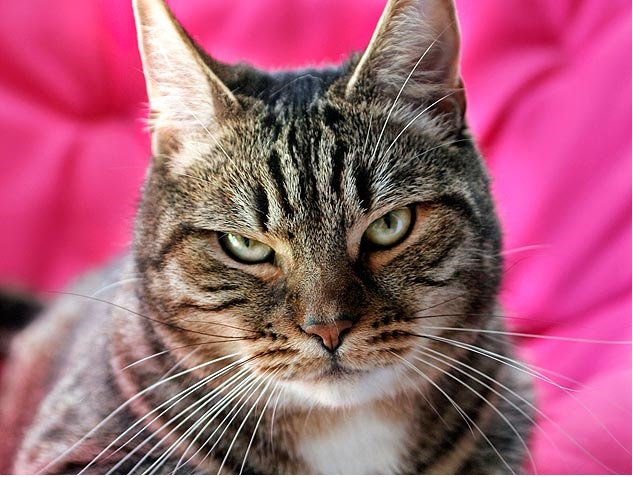
\includegraphics[width=0.5\linewidth]{1a}
    \caption{} 
    \label{1a} 
    \vspace{4ex}
  \end{subfigure}%%
  \begin{subfigure}[b]{0.25\linewidth}
    \centering
    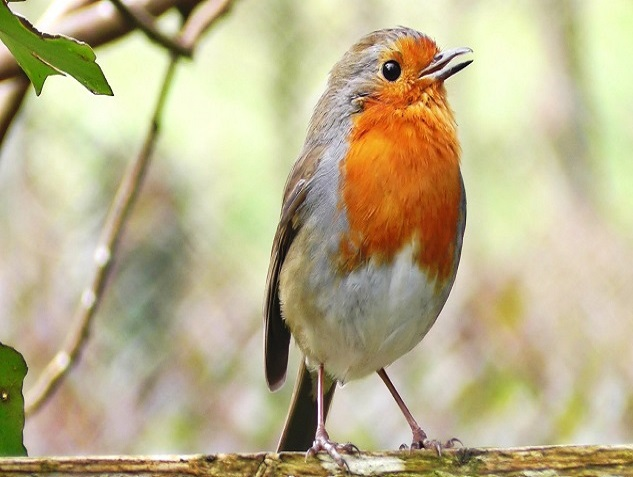
\includegraphics[width=0.5\linewidth]{1b}
    \caption{} 
    \label{1b} 
    \vspace{4ex}
  \end{subfigure}%%
  \begin{subfigure}[b]{0.25\linewidth}
    \centering
    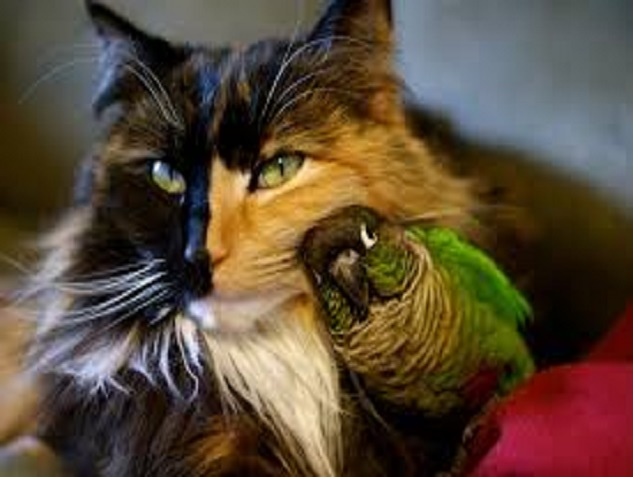
\includegraphics[width=0.5\linewidth]{1c} 
    \caption{} 
    \label{1c} 
    \vspace{4ex}
  \end{subfigure}%%
  \begin{subfigure}[b]{0.25\linewidth}
    \centering
    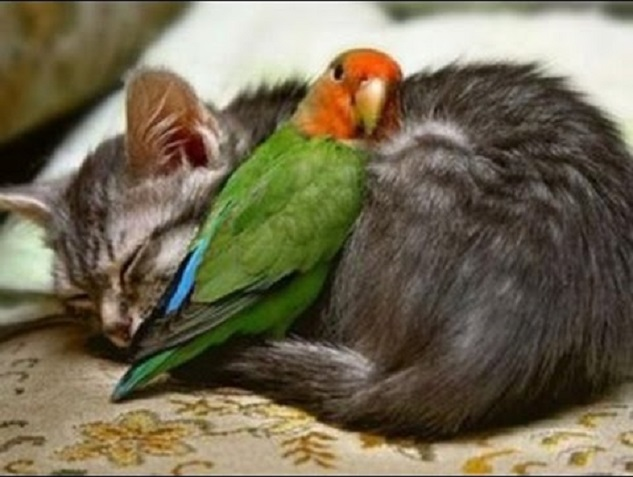
\includegraphics[width=0.5\linewidth]{1d} 
    \caption{} 
    \label{1d}
    \vspace{4ex} 
    \end{subfigure}
  \caption{(a),(b)Some examples from CIFAR-10 \cite{17}. The objects in single-label
images are usually roughly aligned.(c),(d) However, the assumption of object alignment is not valid for multi-label
images. Also note the partial visibility and occlusion
between objects in the multi-label images.}
  \label{fig1} 
\end{figure}

\section{Motivation}
The major, recurrent theme throughout this work is our search for a good generative model for labeling of natural
images. In addition, we seek a model with image segmentation based on objectness measure and selective search that is capable of extracting multiple labels from images. The hope is that we would find out a simple model that can classify multiple labels. Finally, the training time for the model would be small and segmenting the images would be easy enough.

\section{Problem Statement}\label{sec:ProbStatement}
Being able to automatically detect the multiple labels of an
image is a very
challenging task, but it could have great impact, for instance
by helping visually impaired people better identify the
content of images on the web. This task is significantly
harder, for example, than the well-studied image classification or object recognition tasks, which have been a main
focus in the computer vision community. It is also very tough to get dataset of multiple images and train it for a model. That model will be huge and will take loads of time. So our task will be as follows:

% List items using numbering
\begin{enumerate}
  \item To predict a single label image.
  \item Segmentation of an image containing multiple objects into some segmented images using objectness measure \cite{15} and selective search \cite{16}.
  \item Using the segmented images to predict multiple labels in an image. 
\end{enumerate}


\section{Objectives}
% List items using bullets

\begin{itemize}
  \item First objective is to maximize the accuracy of single-label image detection using Convolutional Neural Network(CNN).
  \item Next objective is to produce image windows from an image having multiple objects using objectness measure and selective search.
  \item Last objective is to predict labels of an image using top-1, top-2, total score sum and cumulative percentage sum of the score of every segmented images.
\end{itemize}


